\subsection*{Stage 10-B: Grand Prix of Kyoto, Div 2}
\begin{center}
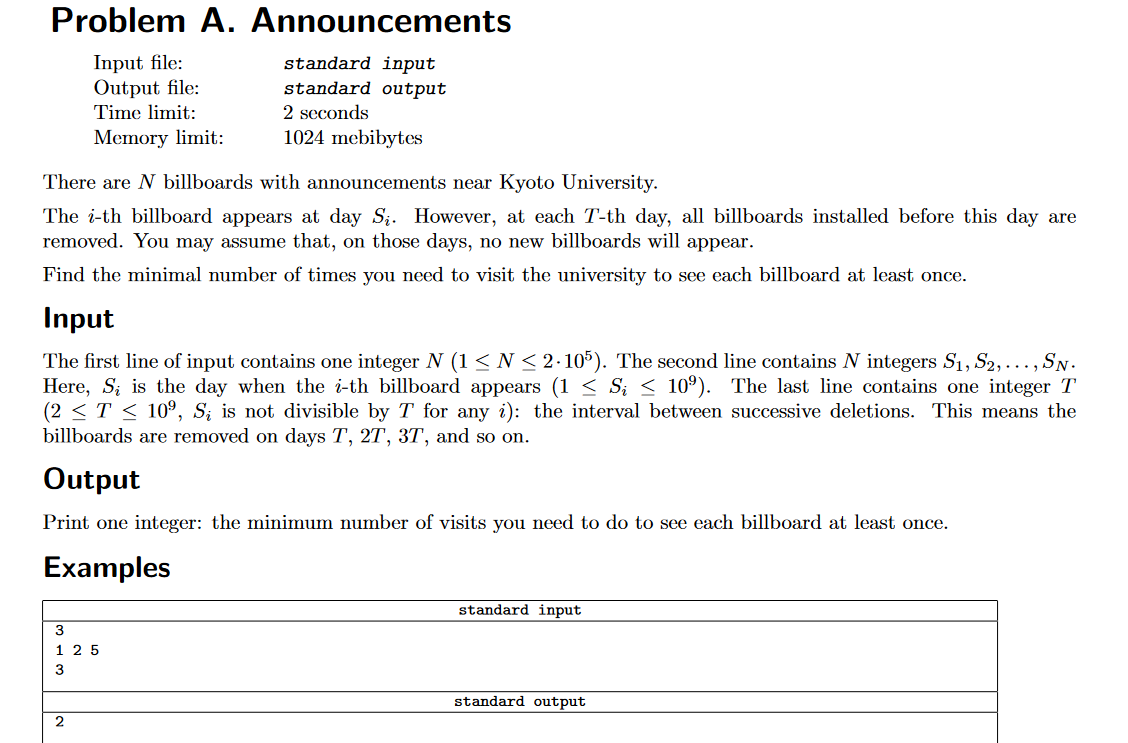
\includegraphics[width=\textwidth]{17A.png}
\end{center}
\subsubsection*{Идея решения}
Пусть одна итерация - это момент от предущего удаления листовок до следующего. Тогда мы можем узнать в какую итерацию была удалена каждая из листовок, поделив день вывешивания листовки на период их удаления. Нам надо узнать кол-во различных итераций. Это легко сделать, если мы результат деления положим в объект типа set и узнаем размер полученного множества. 
\subsubsection*{Исходный код}
\begin{lstlisting}
#include <iostream>
#include <cmath>
#include <vector>
#include <algorithm>
#include <set>
#include <queue>
#include <tuple>
#include <string>
#include <list>
typedef long long ll;
using namespace std;
const ll inf = INT64_MAX;

ll n, t;
vector<ll> a;

int main() {
	ios_base::sync_with_stdio(false);
	cin.tie(0);
	cout.tie(0);
	cin >> n;
	a.resize(n);
	for (int i = 0; i < n; i++) cin >> a[i];
	cin >> t;
	set<ll> ans;
	for (int i = 0; i < n; i++) {
		ans.insert(a[i] / t);
	}
	cout << ans.size();
	return 0;
}
\end{lstlisting}
\subsubsection*{Фрагмент турнирной таблицы контеста}
\begin{center}
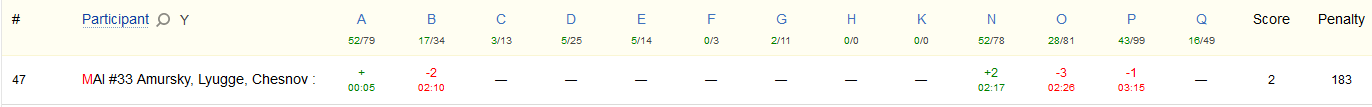
\includegraphics[width=\textwidth]{state17.png}\newline\noindent
\end{center}

\subsubsection*{Выводы}
Задача решена, проблем не возникло. 
